\documentclass[journal]{vgtc} 
\usepackage{hs-vis_ws1819}


%% Please note that the use of figures other than the optional teaser
%% is not permitted on the first page of the journal version.  Figures
%% should begin on the second page and be in CMYK or Grey scale
%% format, otherwise, colour shifting may occur during the printing
%% process.  Papers submitted with figures other than the optional
%% teaser on the first page will be refused.

%% These three lines bring in essential packages: ``mathptmx'' for
%% Type 1 typefaces, ``graphicx'' for inclusion of EPS figures. and
%% ``times'' for proper handling of the times font family.

\usepackage{mathptmx} 
\usepackage{graphicx}
\usepackage{times}
\usepackage[space]{grffile}
\usepackage{pgfplots}
\usepackage[font=normalsize,labelfont=bf]{caption}

%% allow for this line if you want the electronic option to work
%% properly
\vgtcinsertpkg


%% author name
\author{Dominik Sellenthin \and Christian Stegmaier \and Gariharan Kanthasamy}

%% paper title
\title{OpenGL-basiertes Software Occlusion Culling zur Beschleunigung des 3D-Renderings gro{\ss}er Datenmengen und komplexer Szenen}

%% short title for header
\shorttitle{Software Occlusion Culling}


%% Abstract section.
\abstract{%
In Bereichen des 3D-Rendering, sei es in der wissenschaftlichen Visualisierung oder in Computerspielen, ist die Rechenleistung der Grafikkarte schnell an ihrer Grenze, w"ahrend die CPU kaum in Anspruch genommen wird. Damit die GPU entlastet wird, wird ein Software-Rasterisierer eingesetzt, so dass ein Teil der Berechnungen in einem Vorverarbeitungsschritt auf die CPU ausgelagert wird. Um die vollst"andige Rechenleistung moderner Multi-Core CPUs zu gew"ahrleisten, wird in dieser Arbeit ein bereits vorhandener Rasterierer, Mesa 3D, verwendet, der zus"atzlich die OpenGL API zur Verf"ugung stellt. Ziel des Software-Rasterisierers ist es, komplett parallel zum GPU-Rendering des aktuellen Frames, in zwei Schritten festzustellen, welche Objekte in der kommenden Szene zu sehen sind. Im Wesentlichen gilt es dabei zuerst einen geeigneten Tiefenpuffer zu generieren und anschlie{\ss}end mittels Occlusion Queries alle Objekte zu bestimmen, die noch sichtbar sind (auch Z-Buffering genannt). Das Ergebnis der Occlusion Queries kann nun ohne nennenswerte Latenz verwendet werden, um der GPU mitzuteilen, welche Objekte gerendert werden sollen, so dass unn"otiger Rechenaufwand der GPU vermieden wird (~160).
} % end of abstract


%% Uncomment below to include a (optional) teaser figure.
\teaser{ \centering
  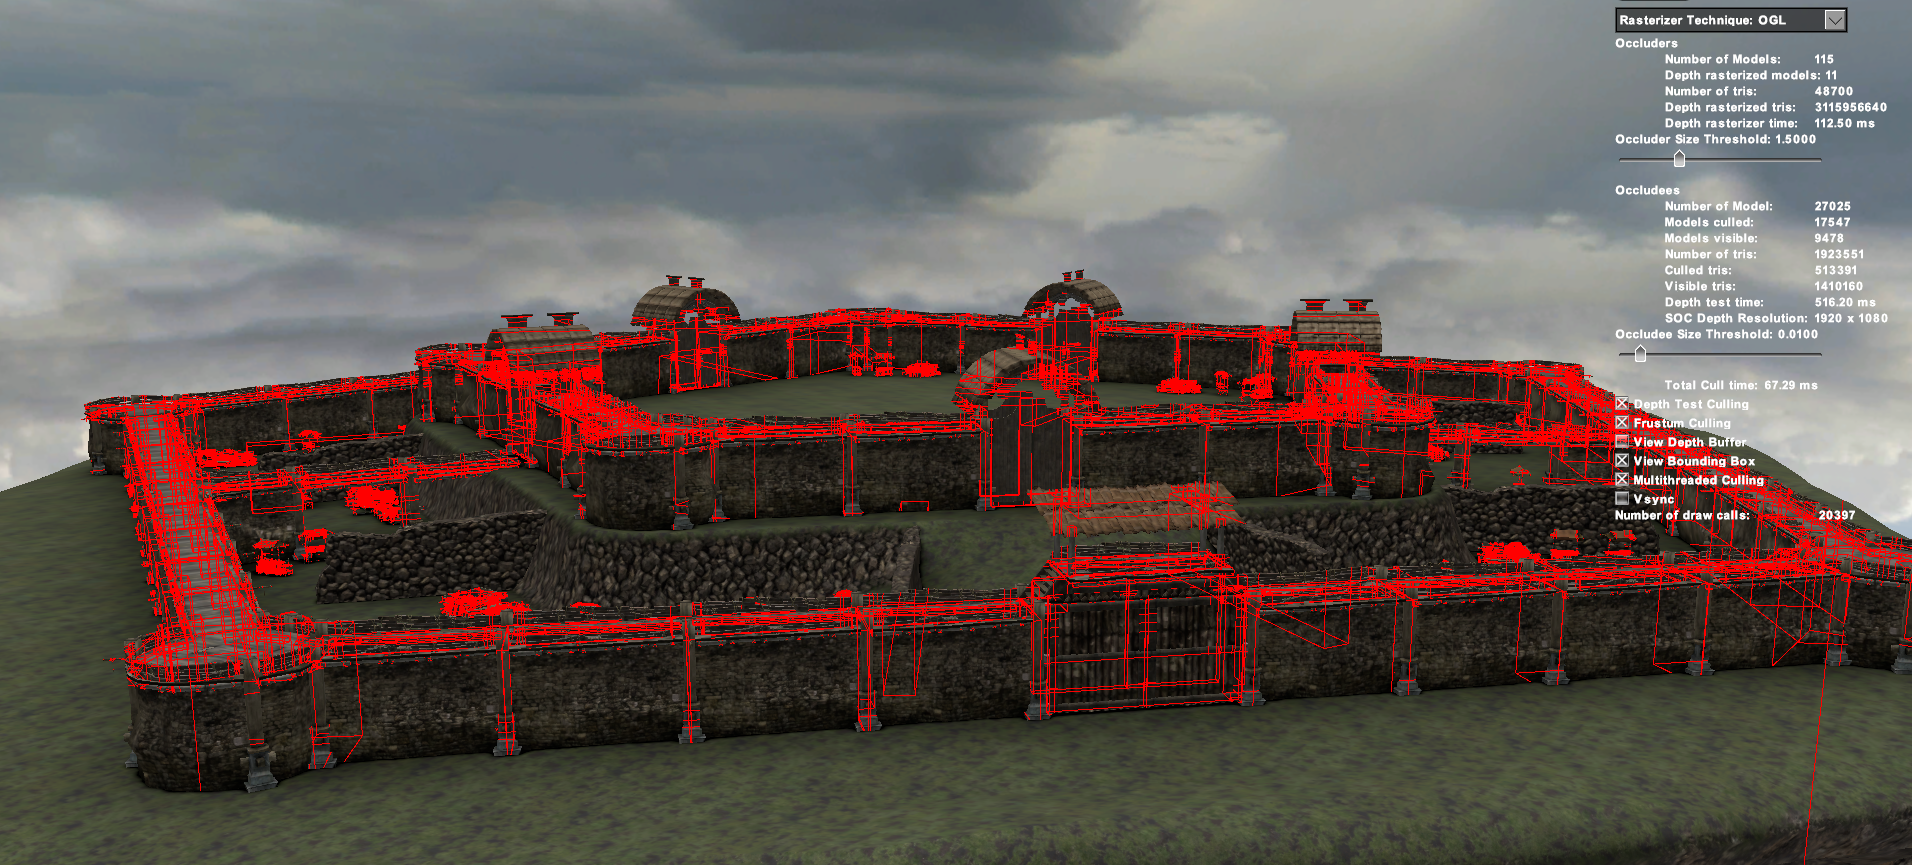
\includegraphics[width=16cm]{images/TeaserScene}
  \caption{Testszene.}
}

%%%%%%%%%%%%%%%%%%%%%%%%%%%%%%%%%%%%%%%%%%%%%%%%%%%%%%%%%%%%%%%%
%%%%%%%%%%%%%%%%%%%%%% START OF THE PAPER %%%%%%%%%%%%%%%%%%%%%%
%%%%%%%%%%%%%%%%%%%%%%%%%%%%%%%%%%%%%%%%%%%%%%%%%%%%%%%%%%%%%%%%

\begin{document}

%% The ``\maketitle'' command must be the first command after the
%% ``\begin{document}'' command. It prepares and prints the title
%%   block.

%%   the only exception to this rule is the \firstsection command
\firstsection{Einleitung}

\maketitle

Egal, ob im Bereich der wissenschaftlichen Visualisierung oder in anderen 3D-Rendering-Bereichen

\section{Related Work}

Das Paper \glqq Masked Software Occlusion Culling \grqq{} von Hasselgren et al. implementiert einen neuen Algorithmus zur Berechnung de hierarchischen Z-Buffers in das Intel Occlusion Culling Framework.
Da heutige Anwendungen immer h"ohere Anspr"uche an die Leistung der Engines stellen wechseln diese von bisherigen Verfahren, wie dem vorherigen berechnen von Mengen die potentiell sichtbar sind, zu Algorithmen die Occluder in einen hierarchischen Z-Buffer rasterisieren.
Der Z-Buffer wird hierbei mit einem Software Rasterisierer berechnet.
Anstatt wie bisher alle Drawcalls an die GPU zu schicken kann nun mit dem Z-Buffer auf der CPU berechnet werden ob ein Occludee von einem Occluder verdeckt wird.
Dadurch kann die Anzahl der Drawcalls an die GPU, unter Verwendung der CPU, verringert werden. In ihrem Paper stellen die Autoren einen Algorithmus vor, der effizient den hierarchischen Z-Buffer berechnen kann und somit die Gesamtperformance entscheidend verbessert.
Anstatt wie in fr"uheren arbeiten Pixel als kleinste Einheit zu betrachten benutzen die Autoren sogenannte Kacheln. Da AVX2 (Advanced Vector Extensions) es erm"oglicht 8 SIMD Instruktionen mit 32-Bit Pr"azision auszuf"uhren wurde f"ur die Kacheln eine Gr"o\ss{}e von 32x8 Pixeln gew"ahlt.
Indem Bitmasken von rechts und links in die Kacheln geschoben werden wird am Ende eine Abdeckungsmaske erhalten, die angibt welche Pixel in einer Kachel verdeckt werden.
W"ahrend ihr Algorithmus keine 100\% Pr"azision garantiert, False Positives sind m"oglich, bewegt sich der Fehler in gleicher Gr"o\ss{}enordnugn wie bei bisherigen Algorithmen.
Ein wichtiger Faktor f"ur die Performance ihres Algorithmus ist die Reihenfolge in der die Objekte gerendert werden, die Objekte werden von vorne nach hinten gerendert.
Durch diese Reihenfolge werden die wichtigsten Occluder als erstes dargestellt und f"ur den Fall, dass die Occlusion Culling Time begrenzt ist, wird trotzdem ein nahezu optimales Ergebnis erzielt.

Als Basiswert f"ur die Performance des Masked Occlusion Algorithmus (MOC) wurde ein normales Rendering ohne Occlusion Culling, aber mit Frustum Culling verwendet.
Frustum Culling rendert nur Objekte die sich im Sichtbereich der Kamera befinden und kann somit je nach Kameraposition einen Teil der Objekte cullen.
Als alternativer Algorithmus wird der \glqq Hierarchical Z Buffer algorithm \grqq{} (HiZ) evaluiert.
Alles Messungen wurden mit voller Aufl"osung (1920*1080 Pixel) ausgef"uhrt, au\ss{}erdem wurde nur die Single-Core Performance betrachtet.
Der MOC Algorithmus ist im Vergleich zum HiZ Algorithmus etwas vorsichtiger und cullt 2\% weniger Dreiecke, erreicht allerdings trotzdem eine bessere Performance.
Bei einem ersten Test mit einer kleinen Kamerafahrt im Intel Occlusion Culling Framework wurde die Framezeit, also die Zeit f"ur die Berechnung eines Frames gemessen.
Szene enth"alt 49k Dreieckige Occluder meshes.
W"ahrend die Performance des Frustum Cullings sehr konstant bleibt, erkennt man bei den beiden Occlusion Culling Algorithmen gr"o\ss{}ere Schwankungen, da ein gro\ss{}er Occluder im Vordergrund potenziell alle Occludees hinter ihm "uberdecken kann und damit die Berechnung stark vereinfacht.
Mit den Occlusion Culling Algorithmen kann eine 1,5-7x schnellere Total Frame Time erreicht werden.
Sind die Berechnungen sehr einfach und es k"onnen sehr viele Objekte gecullt werden, ist die Performance von HiZ und MOC sehr gut und fast identisch.
Je komplexer die Berechnungen sind und je genauer alle Objekte auf potenzielles culling "uberpr"uft werden m"ussen, desto besser schneidet der MOC Algorithmus ab.
In einzelnen Frames erreicht er so teilweise eine etwas mehr als doppelt so schneller Total Frame Time.
In einem zweiten Test wurde eine wesentlich komplexere Szene mit 143k Occluder meshes f"ur die Messung der Daten benutzt.
Die Occlusion Culling Time des MOC Algorithmus ist ca. 10x so schnell wie die des HiZ Algorithmus.
Die Autoren halten fest, dass eine 10-fache Beschleunigung durch ihren Algorithmus vermutlich nicht immer angenommen werden kann, ihr Algorithmus jedoch sehr robust gegen"uber komplexen Occluder Strukturen ist.
Um die Skalierbarkeit des MOC Algorithmus zu testen wurden 32k zuf"allige Occluder Dreiecke mit unterschiedlicher Gr"o\ss{}e erzeugt.
W"ahrend die Performance bei einer Gr"o\ss{}e der Dreiecke von 10x10 praktisch identisch ist, gewinnt der MOC Algorithmus im Vergleich zum HiZ Algorithmus mit steigende Gr"o\ss{}e der Dreiecke immer mehr an Abstand.
Als Endergebnis halten sie fest, dass ihr Algorithmus 3x schneller ist als die bisherigen Algorithmen und gleichzeitig nur einen geringen Memory Overhead hat.
Mit ihrem Algorithmus k"onnen 98\% aller Dreiecke gecullt werden. 



Intel Paper \cite{hpg.20161189}\\
SSE, AVX und maskedAVX\\


\section{Software Occlusion Culling}
Die Menge der Objekte, die es zu Rendern gilt, wird in zwei Mengen aufgeteilt. Zum einen gibt es die Occluder. Occluder sind eine Menge von Objekten, die gro\ss{} genug sind, dass es wahrscheinlich ist, dass sie andere Objekte verdecken. Zum anderen gibt es Occludees. Occludees sind all diejenigen Objekte die potentiell von Occludern verdeckt werden (das hei\ss{}t, sie beinhalten ebenfalls alle Occluder). Sowohl Occluder als auch Occludees liegen dabei in zwei Formen vor. Einmal als Mesh, das zur genauen Darstellung des Objekts in der gerenderten Szene dient und einmal in Form einer Axis Aligned Bounding Box (AABB), die sowohl zum Frustumculling als auch zum (Tiefen-)Rasterisieren verwendet wird. AABBs eignen sich wegen ihrer einfachen geometrischen Form sehr gut, um erste (grobe) Tests durchzuführen, ob ein Objekt überhaupt von der Kamera gesehen werden kann (Frustumculling) und dementsprechend für die folgende Rasterisierung beim Culling in Frage kommt.

FrustumCulling bevor jedem Schritt

Occlusion Culling besteht im Wesentlichen aus zwei Schritten. Als erstes wird der Tiefenpuffer auf Basis einer Occludermenge beschrieben. Occluder sind hierbei alle Objekte,  (Occludees). Diese Occluder werden in einem ersten Renderingdurchlauf, allerdings ohne die Objekte zu zeichnen, rasterisiert und der Tiefenpuffer wird entsprechend der Occludermenge beschrieben.\\
Schritt zwei besteht darin Occlusion Queries durchzuführen. Bei den Occlusion Queries werden die Bounding Boxes aller Occludees gegen den im vorherigen Schritt erstellten Tiefenpuffer getestet und es wird geprüft, ob die Occludees den Tiefentest bestehen oder nicht, sprich, ob die Occludees von einem Occluder verdeckt werden oder sichtbar sind. 

OcclusionQuery

\section{Ergebnisse}
Das ist ein Testsatz f"ur Ergebnisse.
\clearpage

\newpage
\begin{figure}
	\centering
	\begin{minipage}{0.5\textwidth}	
		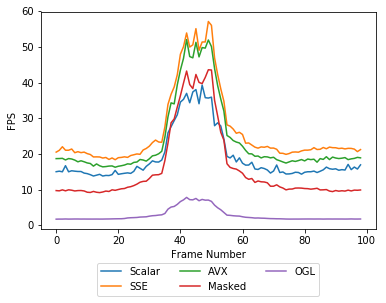
\includegraphics[width=\textwidth]{images/Evaluation_1_Results_FPS.png}
		\caption{Frame Number PNG}
	\end{minipage}
\end{figure}

-
\newpage
-
	
\begin{figure}
	\begin{minipage}{0.5\textwidth}
		%% Creator: Matplotlib, PGF backend
%%
%% To include the figure in your LaTeX document, write
%%   \input{<filename>.pgf}
%%
%% Make sure the required packages are loaded in your preamble
%%   \usepackage{pgf}
%%
%% Figures using additional raster images can only be included by \input if
%% they are in the same directory as the main LaTeX file. For loading figures
%% from other directories you can use the `import` package
%%   \usepackage{import}
%% and then include the figures with
%%   \import{<path to file>}{<filename>.pgf}
%%
%% Matplotlib used the following preamble
%%   \usepackage{fontspec}
%%
\begingroup%
\makeatletter%
\begin{pgfpicture}%
\pgfpathrectangle{\pgfpointorigin}{\pgfqpoint{3.300000in}{2.039555in}}%
\pgfusepath{use as bounding box, clip}%
\begin{pgfscope}%
\pgfsetbuttcap%
\pgfsetmiterjoin%
\definecolor{currentfill}{rgb}{1.000000,1.000000,1.000000}%
\pgfsetfillcolor{currentfill}%
\pgfsetlinewidth{0.000000pt}%
\definecolor{currentstroke}{rgb}{1.000000,1.000000,1.000000}%
\pgfsetstrokecolor{currentstroke}%
\pgfsetdash{}{0pt}%
\pgfpathmoveto{\pgfqpoint{0.000000in}{0.000000in}}%
\pgfpathlineto{\pgfqpoint{3.300000in}{0.000000in}}%
\pgfpathlineto{\pgfqpoint{3.300000in}{2.039555in}}%
\pgfpathlineto{\pgfqpoint{0.000000in}{2.039555in}}%
\pgfpathclose%
\pgfusepath{fill}%
\end{pgfscope}%
\begin{pgfscope}%
\pgfsetbuttcap%
\pgfsetmiterjoin%
\definecolor{currentfill}{rgb}{1.000000,1.000000,1.000000}%
\pgfsetfillcolor{currentfill}%
\pgfsetlinewidth{0.000000pt}%
\definecolor{currentstroke}{rgb}{0.000000,0.000000,0.000000}%
\pgfsetstrokecolor{currentstroke}%
\pgfsetstrokeopacity{0.000000}%
\pgfsetdash{}{0pt}%
\pgfpathmoveto{\pgfqpoint{0.594000in}{0.448702in}}%
\pgfpathlineto{\pgfqpoint{2.970000in}{0.448702in}}%
\pgfpathlineto{\pgfqpoint{2.970000in}{1.794808in}}%
\pgfpathlineto{\pgfqpoint{0.594000in}{1.794808in}}%
\pgfpathclose%
\pgfusepath{fill}%
\end{pgfscope}%
\begin{pgfscope}%
\pgfsetbuttcap%
\pgfsetroundjoin%
\definecolor{currentfill}{rgb}{0.000000,0.000000,0.000000}%
\pgfsetfillcolor{currentfill}%
\pgfsetlinewidth{0.803000pt}%
\definecolor{currentstroke}{rgb}{0.000000,0.000000,0.000000}%
\pgfsetstrokecolor{currentstroke}%
\pgfsetdash{}{0pt}%
\pgfsys@defobject{currentmarker}{\pgfqpoint{0.000000in}{-0.048611in}}{\pgfqpoint{0.000000in}{0.000000in}}{%
\pgfpathmoveto{\pgfqpoint{0.000000in}{0.000000in}}%
\pgfpathlineto{\pgfqpoint{0.000000in}{-0.048611in}}%
\pgfusepath{stroke,fill}%
}%
\begin{pgfscope}%
\pgfsys@transformshift{0.702000in}{0.448702in}%
\pgfsys@useobject{currentmarker}{}%
\end{pgfscope}%
\end{pgfscope}%
\begin{pgfscope}%
\definecolor{textcolor}{rgb}{0.000000,0.000000,0.000000}%
\pgfsetstrokecolor{textcolor}%
\pgfsetfillcolor{textcolor}%
\pgftext[x=0.702000in,y=0.351480in,,top]{\color{textcolor}\rmfamily\fontsize{9.000000}{10.800000}\selectfont 0}%
\end{pgfscope}%
\begin{pgfscope}%
\pgfsetbuttcap%
\pgfsetroundjoin%
\definecolor{currentfill}{rgb}{0.000000,0.000000,0.000000}%
\pgfsetfillcolor{currentfill}%
\pgfsetlinewidth{0.803000pt}%
\definecolor{currentstroke}{rgb}{0.000000,0.000000,0.000000}%
\pgfsetstrokecolor{currentstroke}%
\pgfsetdash{}{0pt}%
\pgfsys@defobject{currentmarker}{\pgfqpoint{0.000000in}{-0.048611in}}{\pgfqpoint{0.000000in}{0.000000in}}{%
\pgfpathmoveto{\pgfqpoint{0.000000in}{0.000000in}}%
\pgfpathlineto{\pgfqpoint{0.000000in}{-0.048611in}}%
\pgfusepath{stroke,fill}%
}%
\begin{pgfscope}%
\pgfsys@transformshift{1.142816in}{0.448702in}%
\pgfsys@useobject{currentmarker}{}%
\end{pgfscope}%
\end{pgfscope}%
\begin{pgfscope}%
\definecolor{textcolor}{rgb}{0.000000,0.000000,0.000000}%
\pgfsetstrokecolor{textcolor}%
\pgfsetfillcolor{textcolor}%
\pgftext[x=1.142816in,y=0.351480in,,top]{\color{textcolor}\rmfamily\fontsize{9.000000}{10.800000}\selectfont 20}%
\end{pgfscope}%
\begin{pgfscope}%
\pgfsetbuttcap%
\pgfsetroundjoin%
\definecolor{currentfill}{rgb}{0.000000,0.000000,0.000000}%
\pgfsetfillcolor{currentfill}%
\pgfsetlinewidth{0.803000pt}%
\definecolor{currentstroke}{rgb}{0.000000,0.000000,0.000000}%
\pgfsetstrokecolor{currentstroke}%
\pgfsetdash{}{0pt}%
\pgfsys@defobject{currentmarker}{\pgfqpoint{0.000000in}{-0.048611in}}{\pgfqpoint{0.000000in}{0.000000in}}{%
\pgfpathmoveto{\pgfqpoint{0.000000in}{0.000000in}}%
\pgfpathlineto{\pgfqpoint{0.000000in}{-0.048611in}}%
\pgfusepath{stroke,fill}%
}%
\begin{pgfscope}%
\pgfsys@transformshift{1.583633in}{0.448702in}%
\pgfsys@useobject{currentmarker}{}%
\end{pgfscope}%
\end{pgfscope}%
\begin{pgfscope}%
\definecolor{textcolor}{rgb}{0.000000,0.000000,0.000000}%
\pgfsetstrokecolor{textcolor}%
\pgfsetfillcolor{textcolor}%
\pgftext[x=1.583633in,y=0.351480in,,top]{\color{textcolor}\rmfamily\fontsize{9.000000}{10.800000}\selectfont 40}%
\end{pgfscope}%
\begin{pgfscope}%
\pgfsetbuttcap%
\pgfsetroundjoin%
\definecolor{currentfill}{rgb}{0.000000,0.000000,0.000000}%
\pgfsetfillcolor{currentfill}%
\pgfsetlinewidth{0.803000pt}%
\definecolor{currentstroke}{rgb}{0.000000,0.000000,0.000000}%
\pgfsetstrokecolor{currentstroke}%
\pgfsetdash{}{0pt}%
\pgfsys@defobject{currentmarker}{\pgfqpoint{0.000000in}{-0.048611in}}{\pgfqpoint{0.000000in}{0.000000in}}{%
\pgfpathmoveto{\pgfqpoint{0.000000in}{0.000000in}}%
\pgfpathlineto{\pgfqpoint{0.000000in}{-0.048611in}}%
\pgfusepath{stroke,fill}%
}%
\begin{pgfscope}%
\pgfsys@transformshift{2.024449in}{0.448702in}%
\pgfsys@useobject{currentmarker}{}%
\end{pgfscope}%
\end{pgfscope}%
\begin{pgfscope}%
\definecolor{textcolor}{rgb}{0.000000,0.000000,0.000000}%
\pgfsetstrokecolor{textcolor}%
\pgfsetfillcolor{textcolor}%
\pgftext[x=2.024449in,y=0.351480in,,top]{\color{textcolor}\rmfamily\fontsize{9.000000}{10.800000}\selectfont 60}%
\end{pgfscope}%
\begin{pgfscope}%
\pgfsetbuttcap%
\pgfsetroundjoin%
\definecolor{currentfill}{rgb}{0.000000,0.000000,0.000000}%
\pgfsetfillcolor{currentfill}%
\pgfsetlinewidth{0.803000pt}%
\definecolor{currentstroke}{rgb}{0.000000,0.000000,0.000000}%
\pgfsetstrokecolor{currentstroke}%
\pgfsetdash{}{0pt}%
\pgfsys@defobject{currentmarker}{\pgfqpoint{0.000000in}{-0.048611in}}{\pgfqpoint{0.000000in}{0.000000in}}{%
\pgfpathmoveto{\pgfqpoint{0.000000in}{0.000000in}}%
\pgfpathlineto{\pgfqpoint{0.000000in}{-0.048611in}}%
\pgfusepath{stroke,fill}%
}%
\begin{pgfscope}%
\pgfsys@transformshift{2.465265in}{0.448702in}%
\pgfsys@useobject{currentmarker}{}%
\end{pgfscope}%
\end{pgfscope}%
\begin{pgfscope}%
\definecolor{textcolor}{rgb}{0.000000,0.000000,0.000000}%
\pgfsetstrokecolor{textcolor}%
\pgfsetfillcolor{textcolor}%
\pgftext[x=2.465265in,y=0.351480in,,top]{\color{textcolor}\rmfamily\fontsize{9.000000}{10.800000}\selectfont 80}%
\end{pgfscope}%
\begin{pgfscope}%
\pgfsetbuttcap%
\pgfsetroundjoin%
\definecolor{currentfill}{rgb}{0.000000,0.000000,0.000000}%
\pgfsetfillcolor{currentfill}%
\pgfsetlinewidth{0.803000pt}%
\definecolor{currentstroke}{rgb}{0.000000,0.000000,0.000000}%
\pgfsetstrokecolor{currentstroke}%
\pgfsetdash{}{0pt}%
\pgfsys@defobject{currentmarker}{\pgfqpoint{0.000000in}{-0.048611in}}{\pgfqpoint{0.000000in}{0.000000in}}{%
\pgfpathmoveto{\pgfqpoint{0.000000in}{0.000000in}}%
\pgfpathlineto{\pgfqpoint{0.000000in}{-0.048611in}}%
\pgfusepath{stroke,fill}%
}%
\begin{pgfscope}%
\pgfsys@transformshift{2.906082in}{0.448702in}%
\pgfsys@useobject{currentmarker}{}%
\end{pgfscope}%
\end{pgfscope}%
\begin{pgfscope}%
\definecolor{textcolor}{rgb}{0.000000,0.000000,0.000000}%
\pgfsetstrokecolor{textcolor}%
\pgfsetfillcolor{textcolor}%
\pgftext[x=2.906082in,y=0.351480in,,top]{\color{textcolor}\rmfamily\fontsize{9.000000}{10.800000}\selectfont 100}%
\end{pgfscope}%
\begin{pgfscope}%
\definecolor{textcolor}{rgb}{0.000000,0.000000,0.000000}%
\pgfsetstrokecolor{textcolor}%
\pgfsetfillcolor{textcolor}%
\pgftext[x=1.782000in,y=0.184924in,,top]{\color{textcolor}\rmfamily\fontsize{9.000000}{10.800000}\selectfont Frame Number}%
\end{pgfscope}%
\begin{pgfscope}%
\pgfsetbuttcap%
\pgfsetroundjoin%
\definecolor{currentfill}{rgb}{0.000000,0.000000,0.000000}%
\pgfsetfillcolor{currentfill}%
\pgfsetlinewidth{0.803000pt}%
\definecolor{currentstroke}{rgb}{0.000000,0.000000,0.000000}%
\pgfsetstrokecolor{currentstroke}%
\pgfsetdash{}{0pt}%
\pgfsys@defobject{currentmarker}{\pgfqpoint{-0.048611in}{0.000000in}}{\pgfqpoint{0.000000in}{0.000000in}}{%
\pgfpathmoveto{\pgfqpoint{0.000000in}{0.000000in}}%
\pgfpathlineto{\pgfqpoint{-0.048611in}{0.000000in}}%
\pgfusepath{stroke,fill}%
}%
\begin{pgfscope}%
\pgfsys@transformshift{0.594000in}{0.470992in}%
\pgfsys@useobject{currentmarker}{}%
\end{pgfscope}%
\end{pgfscope}%
\begin{pgfscope}%
\definecolor{textcolor}{rgb}{0.000000,0.000000,0.000000}%
\pgfsetstrokecolor{textcolor}%
\pgfsetfillcolor{textcolor}%
\pgftext[x=0.432528in,y=0.427617in,left,base]{\color{textcolor}\rmfamily\fontsize{9.000000}{10.800000}\selectfont 0}%
\end{pgfscope}%
\begin{pgfscope}%
\pgfsetbuttcap%
\pgfsetroundjoin%
\definecolor{currentfill}{rgb}{0.000000,0.000000,0.000000}%
\pgfsetfillcolor{currentfill}%
\pgfsetlinewidth{0.803000pt}%
\definecolor{currentstroke}{rgb}{0.000000,0.000000,0.000000}%
\pgfsetstrokecolor{currentstroke}%
\pgfsetdash{}{0pt}%
\pgfsys@defobject{currentmarker}{\pgfqpoint{-0.048611in}{0.000000in}}{\pgfqpoint{0.000000in}{0.000000in}}{%
\pgfpathmoveto{\pgfqpoint{0.000000in}{0.000000in}}%
\pgfpathlineto{\pgfqpoint{-0.048611in}{0.000000in}}%
\pgfusepath{stroke,fill}%
}%
\begin{pgfscope}%
\pgfsys@transformshift{0.594000in}{0.913117in}%
\pgfsys@useobject{currentmarker}{}%
\end{pgfscope}%
\end{pgfscope}%
\begin{pgfscope}%
\definecolor{textcolor}{rgb}{0.000000,0.000000,0.000000}%
\pgfsetstrokecolor{textcolor}%
\pgfsetfillcolor{textcolor}%
\pgftext[x=0.368278in,y=0.869742in,left,base]{\color{textcolor}\rmfamily\fontsize{9.000000}{10.800000}\selectfont 20}%
\end{pgfscope}%
\begin{pgfscope}%
\pgfsetbuttcap%
\pgfsetroundjoin%
\definecolor{currentfill}{rgb}{0.000000,0.000000,0.000000}%
\pgfsetfillcolor{currentfill}%
\pgfsetlinewidth{0.803000pt}%
\definecolor{currentstroke}{rgb}{0.000000,0.000000,0.000000}%
\pgfsetstrokecolor{currentstroke}%
\pgfsetdash{}{0pt}%
\pgfsys@defobject{currentmarker}{\pgfqpoint{-0.048611in}{0.000000in}}{\pgfqpoint{0.000000in}{0.000000in}}{%
\pgfpathmoveto{\pgfqpoint{0.000000in}{0.000000in}}%
\pgfpathlineto{\pgfqpoint{-0.048611in}{0.000000in}}%
\pgfusepath{stroke,fill}%
}%
\begin{pgfscope}%
\pgfsys@transformshift{0.594000in}{1.355242in}%
\pgfsys@useobject{currentmarker}{}%
\end{pgfscope}%
\end{pgfscope}%
\begin{pgfscope}%
\definecolor{textcolor}{rgb}{0.000000,0.000000,0.000000}%
\pgfsetstrokecolor{textcolor}%
\pgfsetfillcolor{textcolor}%
\pgftext[x=0.368278in,y=1.311867in,left,base]{\color{textcolor}\rmfamily\fontsize{9.000000}{10.800000}\selectfont 40}%
\end{pgfscope}%
\begin{pgfscope}%
\pgfsetbuttcap%
\pgfsetroundjoin%
\definecolor{currentfill}{rgb}{0.000000,0.000000,0.000000}%
\pgfsetfillcolor{currentfill}%
\pgfsetlinewidth{0.803000pt}%
\definecolor{currentstroke}{rgb}{0.000000,0.000000,0.000000}%
\pgfsetstrokecolor{currentstroke}%
\pgfsetdash{}{0pt}%
\pgfsys@defobject{currentmarker}{\pgfqpoint{-0.048611in}{0.000000in}}{\pgfqpoint{0.000000in}{0.000000in}}{%
\pgfpathmoveto{\pgfqpoint{0.000000in}{0.000000in}}%
\pgfpathlineto{\pgfqpoint{-0.048611in}{0.000000in}}%
\pgfusepath{stroke,fill}%
}%
\begin{pgfscope}%
\pgfsys@transformshift{0.594000in}{1.797367in}%
\pgfsys@useobject{currentmarker}{}%
\end{pgfscope}%
\end{pgfscope}%
\begin{pgfscope}%
\definecolor{textcolor}{rgb}{0.000000,0.000000,0.000000}%
\pgfsetstrokecolor{textcolor}%
\pgfsetfillcolor{textcolor}%
\pgftext[x=0.368278in,y=1.753992in,left,base]{\color{textcolor}\rmfamily\fontsize{9.000000}{10.800000}\selectfont 60}%
\end{pgfscope}%
\begin{pgfscope}%
\definecolor{textcolor}{rgb}{0.000000,0.000000,0.000000}%
\pgfsetstrokecolor{textcolor}%
\pgfsetfillcolor{textcolor}%
\pgftext[x=0.312722in,y=1.121755in,,bottom,rotate=90.000000]{\color{textcolor}\rmfamily\fontsize{9.000000}{10.800000}\selectfont FPS}%
\end{pgfscope}%
\begin{pgfscope}%
\pgfpathrectangle{\pgfqpoint{0.594000in}{0.448702in}}{\pgfqpoint{2.376000in}{1.346106in}}%
\pgfusepath{clip}%
\pgfsetrectcap%
\pgfsetroundjoin%
\pgfsetlinewidth{1.505625pt}%
\definecolor{currentstroke}{rgb}{0.121569,0.466667,0.705882}%
\pgfsetstrokecolor{currentstroke}%
\pgfsetdash{}{0pt}%
\pgfpathmoveto{\pgfqpoint{0.702000in}{0.803705in}}%
\pgfpathlineto{\pgfqpoint{0.724041in}{0.806930in}}%
\pgfpathlineto{\pgfqpoint{0.746082in}{0.803161in}}%
\pgfpathlineto{\pgfqpoint{0.768122in}{0.840903in}}%
\pgfpathlineto{\pgfqpoint{0.790163in}{0.803198in}}%
\pgfpathlineto{\pgfqpoint{0.812204in}{0.809503in}}%
\pgfpathlineto{\pgfqpoint{0.834245in}{0.806895in}}%
\pgfpathlineto{\pgfqpoint{0.856286in}{0.805058in}}%
\pgfpathlineto{\pgfqpoint{0.878327in}{0.804881in}}%
\pgfpathlineto{\pgfqpoint{0.900367in}{0.795074in}}%
\pgfpathlineto{\pgfqpoint{0.922408in}{0.791805in}}%
\pgfpathlineto{\pgfqpoint{0.944449in}{0.785235in}}%
\pgfpathlineto{\pgfqpoint{0.966490in}{0.777007in}}%
\pgfpathlineto{\pgfqpoint{0.988531in}{0.782164in}}%
\pgfpathlineto{\pgfqpoint{1.010571in}{0.787503in}}%
\pgfpathlineto{\pgfqpoint{1.032612in}{0.776848in}}%
\pgfpathlineto{\pgfqpoint{1.054653in}{0.780741in}}%
\pgfpathlineto{\pgfqpoint{1.076694in}{0.779830in}}%
\pgfpathlineto{\pgfqpoint{1.098735in}{0.785639in}}%
\pgfpathlineto{\pgfqpoint{1.120776in}{0.811833in}}%
\pgfpathlineto{\pgfqpoint{1.142816in}{0.787399in}}%
\pgfpathlineto{\pgfqpoint{1.164857in}{0.790947in}}%
\pgfpathlineto{\pgfqpoint{1.186898in}{0.793918in}}%
\pgfpathlineto{\pgfqpoint{1.208939in}{0.796476in}}%
\pgfpathlineto{\pgfqpoint{1.230980in}{0.793282in}}%
\pgfpathlineto{\pgfqpoint{1.253020in}{0.806105in}}%
\pgfpathlineto{\pgfqpoint{1.275061in}{0.836835in}}%
\pgfpathlineto{\pgfqpoint{1.297102in}{0.824856in}}%
\pgfpathlineto{\pgfqpoint{1.319143in}{0.813098in}}%
\pgfpathlineto{\pgfqpoint{1.341184in}{0.836658in}}%
\pgfpathlineto{\pgfqpoint{1.363224in}{0.851892in}}%
\pgfpathlineto{\pgfqpoint{1.385265in}{0.870837in}}%
\pgfpathlineto{\pgfqpoint{1.407306in}{0.864103in}}%
\pgfpathlineto{\pgfqpoint{1.429347in}{0.863416in}}%
\pgfpathlineto{\pgfqpoint{1.451388in}{0.875727in}}%
\pgfpathlineto{\pgfqpoint{1.473429in}{0.926085in}}%
\pgfpathlineto{\pgfqpoint{1.495469in}{1.044305in}}%
\pgfpathlineto{\pgfqpoint{1.517510in}{1.082341in}}%
\pgfpathlineto{\pgfqpoint{1.539551in}{1.119890in}}%
\pgfpathlineto{\pgfqpoint{1.561592in}{1.156191in}}%
\pgfpathlineto{\pgfqpoint{1.583633in}{1.234651in}}%
\pgfpathlineto{\pgfqpoint{1.605673in}{1.251613in}}%
\pgfpathlineto{\pgfqpoint{1.627714in}{1.288764in}}%
\pgfpathlineto{\pgfqpoint{1.649755in}{1.230592in}}%
\pgfpathlineto{\pgfqpoint{1.671796in}{1.297388in}}%
\pgfpathlineto{\pgfqpoint{1.693837in}{1.312279in}}%
\pgfpathlineto{\pgfqpoint{1.715878in}{1.224320in}}%
\pgfpathlineto{\pgfqpoint{1.737918in}{1.340146in}}%
\pgfpathlineto{\pgfqpoint{1.759959in}{1.261927in}}%
\pgfpathlineto{\pgfqpoint{1.782000in}{1.259600in}}%
\pgfpathlineto{\pgfqpoint{1.804041in}{1.265162in}}%
\pgfpathlineto{\pgfqpoint{1.826082in}{1.088391in}}%
\pgfpathlineto{\pgfqpoint{1.848122in}{1.106406in}}%
\pgfpathlineto{\pgfqpoint{1.870163in}{1.086813in}}%
\pgfpathlineto{\pgfqpoint{1.892204in}{1.006207in}}%
\pgfpathlineto{\pgfqpoint{1.914245in}{0.898558in}}%
\pgfpathlineto{\pgfqpoint{1.936286in}{0.888898in}}%
\pgfpathlineto{\pgfqpoint{1.958327in}{0.905732in}}%
\pgfpathlineto{\pgfqpoint{1.980367in}{0.863962in}}%
\pgfpathlineto{\pgfqpoint{2.002408in}{0.889517in}}%
\pgfpathlineto{\pgfqpoint{2.024449in}{0.856309in}}%
\pgfpathlineto{\pgfqpoint{2.046490in}{0.844369in}}%
\pgfpathlineto{\pgfqpoint{2.068531in}{0.844860in}}%
\pgfpathlineto{\pgfqpoint{2.090571in}{0.862156in}}%
\pgfpathlineto{\pgfqpoint{2.112612in}{0.820446in}}%
\pgfpathlineto{\pgfqpoint{2.134653in}{0.817685in}}%
\pgfpathlineto{\pgfqpoint{2.156694in}{0.828450in}}%
\pgfpathlineto{\pgfqpoint{2.178735in}{0.823404in}}%
\pgfpathlineto{\pgfqpoint{2.200776in}{0.814271in}}%
\pgfpathlineto{\pgfqpoint{2.222816in}{0.795253in}}%
\pgfpathlineto{\pgfqpoint{2.244857in}{0.807938in}}%
\pgfpathlineto{\pgfqpoint{2.266898in}{0.845154in}}%
\pgfpathlineto{\pgfqpoint{2.288939in}{0.798567in}}%
\pgfpathlineto{\pgfqpoint{2.310980in}{0.802056in}}%
\pgfpathlineto{\pgfqpoint{2.333020in}{0.789572in}}%
\pgfpathlineto{\pgfqpoint{2.355061in}{0.789952in}}%
\pgfpathlineto{\pgfqpoint{2.377102in}{0.792895in}}%
\pgfpathlineto{\pgfqpoint{2.399143in}{0.800287in}}%
\pgfpathlineto{\pgfqpoint{2.421184in}{0.798883in}}%
\pgfpathlineto{\pgfqpoint{2.443224in}{0.788392in}}%
\pgfpathlineto{\pgfqpoint{2.465265in}{0.800148in}}%
\pgfpathlineto{\pgfqpoint{2.487306in}{0.803366in}}%
\pgfpathlineto{\pgfqpoint{2.509347in}{0.803362in}}%
\pgfpathlineto{\pgfqpoint{2.531388in}{0.807476in}}%
\pgfpathlineto{\pgfqpoint{2.553429in}{0.798523in}}%
\pgfpathlineto{\pgfqpoint{2.575469in}{0.806468in}}%
\pgfpathlineto{\pgfqpoint{2.597510in}{0.815333in}}%
\pgfpathlineto{\pgfqpoint{2.619551in}{0.832113in}}%
\pgfpathlineto{\pgfqpoint{2.641592in}{0.822365in}}%
\pgfpathlineto{\pgfqpoint{2.663633in}{0.818934in}}%
\pgfpathlineto{\pgfqpoint{2.685673in}{0.821662in}}%
\pgfpathlineto{\pgfqpoint{2.707714in}{0.812673in}}%
\pgfpathlineto{\pgfqpoint{2.729755in}{0.816383in}}%
\pgfpathlineto{\pgfqpoint{2.751796in}{0.813975in}}%
\pgfpathlineto{\pgfqpoint{2.773837in}{0.848950in}}%
\pgfpathlineto{\pgfqpoint{2.795878in}{0.816551in}}%
\pgfpathlineto{\pgfqpoint{2.817918in}{0.832478in}}%
\pgfpathlineto{\pgfqpoint{2.839959in}{0.820119in}}%
\pgfpathlineto{\pgfqpoint{2.862000in}{0.846078in}}%
\pgfusepath{stroke}%
\end{pgfscope}%
\begin{pgfscope}%
\pgfpathrectangle{\pgfqpoint{0.594000in}{0.448702in}}{\pgfqpoint{2.376000in}{1.346106in}}%
\pgfusepath{clip}%
\pgfsetrectcap%
\pgfsetroundjoin%
\pgfsetlinewidth{1.505625pt}%
\definecolor{currentstroke}{rgb}{1.000000,0.498039,0.054902}%
\pgfsetstrokecolor{currentstroke}%
\pgfsetdash{}{0pt}%
\pgfpathmoveto{\pgfqpoint{0.702000in}{0.924838in}}%
\pgfpathlineto{\pgfqpoint{0.724041in}{0.935938in}}%
\pgfpathlineto{\pgfqpoint{0.746082in}{0.958179in}}%
\pgfpathlineto{\pgfqpoint{0.768122in}{0.936630in}}%
\pgfpathlineto{\pgfqpoint{0.790163in}{0.936548in}}%
\pgfpathlineto{\pgfqpoint{0.812204in}{0.944117in}}%
\pgfpathlineto{\pgfqpoint{0.834245in}{0.921343in}}%
\pgfpathlineto{\pgfqpoint{0.856286in}{0.927610in}}%
\pgfpathlineto{\pgfqpoint{0.878327in}{0.921714in}}%
\pgfpathlineto{\pgfqpoint{0.900367in}{0.924984in}}%
\pgfpathlineto{\pgfqpoint{0.922408in}{0.915695in}}%
\pgfpathlineto{\pgfqpoint{0.944449in}{0.910133in}}%
\pgfpathlineto{\pgfqpoint{0.966490in}{0.895090in}}%
\pgfpathlineto{\pgfqpoint{0.988531in}{0.895543in}}%
\pgfpathlineto{\pgfqpoint{1.010571in}{0.894891in}}%
\pgfpathlineto{\pgfqpoint{1.032612in}{0.888290in}}%
\pgfpathlineto{\pgfqpoint{1.054653in}{0.891721in}}%
\pgfpathlineto{\pgfqpoint{1.076694in}{0.879682in}}%
\pgfpathlineto{\pgfqpoint{1.098735in}{0.888836in}}%
\pgfpathlineto{\pgfqpoint{1.120776in}{0.877878in}}%
\pgfpathlineto{\pgfqpoint{1.142816in}{0.890425in}}%
\pgfpathlineto{\pgfqpoint{1.164857in}{0.892256in}}%
\pgfpathlineto{\pgfqpoint{1.186898in}{0.895775in}}%
\pgfpathlineto{\pgfqpoint{1.208939in}{0.892311in}}%
\pgfpathlineto{\pgfqpoint{1.230980in}{0.903833in}}%
\pgfpathlineto{\pgfqpoint{1.253020in}{0.908566in}}%
\pgfpathlineto{\pgfqpoint{1.275061in}{0.913606in}}%
\pgfpathlineto{\pgfqpoint{1.297102in}{0.911437in}}%
\pgfpathlineto{\pgfqpoint{1.319143in}{0.938000in}}%
\pgfpathlineto{\pgfqpoint{1.341184in}{0.947477in}}%
\pgfpathlineto{\pgfqpoint{1.363224in}{0.961718in}}%
\pgfpathlineto{\pgfqpoint{1.385265in}{0.984076in}}%
\pgfpathlineto{\pgfqpoint{1.407306in}{0.999489in}}%
\pgfpathlineto{\pgfqpoint{1.429347in}{0.987540in}}%
\pgfpathlineto{\pgfqpoint{1.451388in}{0.985560in}}%
\pgfpathlineto{\pgfqpoint{1.473429in}{1.080592in}}%
\pgfpathlineto{\pgfqpoint{1.495469in}{1.220346in}}%
\pgfpathlineto{\pgfqpoint{1.517510in}{1.282862in}}%
\pgfpathlineto{\pgfqpoint{1.539551in}{1.328063in}}%
\pgfpathlineto{\pgfqpoint{1.561592in}{1.404064in}}%
\pgfpathlineto{\pgfqpoint{1.583633in}{1.530914in}}%
\pgfpathlineto{\pgfqpoint{1.605673in}{1.577755in}}%
\pgfpathlineto{\pgfqpoint{1.627714in}{1.662557in}}%
\pgfpathlineto{\pgfqpoint{1.649755in}{1.575498in}}%
\pgfpathlineto{\pgfqpoint{1.671796in}{1.588994in}}%
\pgfpathlineto{\pgfqpoint{1.693837in}{1.689208in}}%
\pgfpathlineto{\pgfqpoint{1.715878in}{1.555313in}}%
\pgfpathlineto{\pgfqpoint{1.737918in}{1.606551in}}%
\pgfpathlineto{\pgfqpoint{1.759959in}{1.607059in}}%
\pgfpathlineto{\pgfqpoint{1.782000in}{1.733622in}}%
\pgfpathlineto{\pgfqpoint{1.804041in}{1.709743in}}%
\pgfpathlineto{\pgfqpoint{1.826082in}{1.508854in}}%
\pgfpathlineto{\pgfqpoint{1.848122in}{1.404984in}}%
\pgfpathlineto{\pgfqpoint{1.870163in}{1.316864in}}%
\pgfpathlineto{\pgfqpoint{1.892204in}{1.240078in}}%
\pgfpathlineto{\pgfqpoint{1.914245in}{1.093542in}}%
\pgfpathlineto{\pgfqpoint{1.936286in}{1.085761in}}%
\pgfpathlineto{\pgfqpoint{1.958327in}{1.067753in}}%
\pgfpathlineto{\pgfqpoint{1.980367in}{1.041709in}}%
\pgfpathlineto{\pgfqpoint{2.002408in}{1.047627in}}%
\pgfpathlineto{\pgfqpoint{2.024449in}{1.034220in}}%
\pgfpathlineto{\pgfqpoint{2.046490in}{0.980203in}}%
\pgfpathlineto{\pgfqpoint{2.068531in}{0.981603in}}%
\pgfpathlineto{\pgfqpoint{2.090571in}{0.968648in}}%
\pgfpathlineto{\pgfqpoint{2.112612in}{0.955654in}}%
\pgfpathlineto{\pgfqpoint{2.134653in}{0.949571in}}%
\pgfpathlineto{\pgfqpoint{2.156694in}{0.957162in}}%
\pgfpathlineto{\pgfqpoint{2.178735in}{0.955035in}}%
\pgfpathlineto{\pgfqpoint{2.200776in}{0.960197in}}%
\pgfpathlineto{\pgfqpoint{2.222816in}{0.949674in}}%
\pgfpathlineto{\pgfqpoint{2.244857in}{0.950092in}}%
\pgfpathlineto{\pgfqpoint{2.266898in}{0.942565in}}%
\pgfpathlineto{\pgfqpoint{2.288939in}{0.918191in}}%
\pgfpathlineto{\pgfqpoint{2.310980in}{0.917492in}}%
\pgfpathlineto{\pgfqpoint{2.333020in}{0.911057in}}%
\pgfpathlineto{\pgfqpoint{2.355061in}{0.915958in}}%
\pgfpathlineto{\pgfqpoint{2.377102in}{0.924593in}}%
\pgfpathlineto{\pgfqpoint{2.399143in}{0.925926in}}%
\pgfpathlineto{\pgfqpoint{2.421184in}{0.924445in}}%
\pgfpathlineto{\pgfqpoint{2.443224in}{0.932489in}}%
\pgfpathlineto{\pgfqpoint{2.465265in}{0.937242in}}%
\pgfpathlineto{\pgfqpoint{2.487306in}{0.937111in}}%
\pgfpathlineto{\pgfqpoint{2.509347in}{0.939627in}}%
\pgfpathlineto{\pgfqpoint{2.531388in}{0.952595in}}%
\pgfpathlineto{\pgfqpoint{2.553429in}{0.941221in}}%
\pgfpathlineto{\pgfqpoint{2.575469in}{0.942317in}}%
\pgfpathlineto{\pgfqpoint{2.597510in}{0.953665in}}%
\pgfpathlineto{\pgfqpoint{2.619551in}{0.945686in}}%
\pgfpathlineto{\pgfqpoint{2.641592in}{0.956019in}}%
\pgfpathlineto{\pgfqpoint{2.663633in}{0.952469in}}%
\pgfpathlineto{\pgfqpoint{2.685673in}{0.952004in}}%
\pgfpathlineto{\pgfqpoint{2.707714in}{0.947172in}}%
\pgfpathlineto{\pgfqpoint{2.729755in}{0.949305in}}%
\pgfpathlineto{\pgfqpoint{2.751796in}{0.944734in}}%
\pgfpathlineto{\pgfqpoint{2.773837in}{0.948306in}}%
\pgfpathlineto{\pgfqpoint{2.795878in}{0.947919in}}%
\pgfpathlineto{\pgfqpoint{2.817918in}{0.943564in}}%
\pgfpathlineto{\pgfqpoint{2.839959in}{0.928081in}}%
\pgfpathlineto{\pgfqpoint{2.862000in}{0.940569in}}%
\pgfusepath{stroke}%
\end{pgfscope}%
\begin{pgfscope}%
\pgfpathrectangle{\pgfqpoint{0.594000in}{0.448702in}}{\pgfqpoint{2.376000in}{1.346106in}}%
\pgfusepath{clip}%
\pgfsetrectcap%
\pgfsetroundjoin%
\pgfsetlinewidth{1.505625pt}%
\definecolor{currentstroke}{rgb}{0.172549,0.627451,0.172549}%
\pgfsetstrokecolor{currentstroke}%
\pgfsetdash{}{0pt}%
\pgfpathmoveto{\pgfqpoint{0.702000in}{0.884653in}}%
\pgfpathlineto{\pgfqpoint{0.724041in}{0.885186in}}%
\pgfpathlineto{\pgfqpoint{0.746082in}{0.886453in}}%
\pgfpathlineto{\pgfqpoint{0.768122in}{0.876509in}}%
\pgfpathlineto{\pgfqpoint{0.790163in}{0.885084in}}%
\pgfpathlineto{\pgfqpoint{0.812204in}{0.882326in}}%
\pgfpathlineto{\pgfqpoint{0.834245in}{0.875537in}}%
\pgfpathlineto{\pgfqpoint{0.856286in}{0.864970in}}%
\pgfpathlineto{\pgfqpoint{0.878327in}{0.871286in}}%
\pgfpathlineto{\pgfqpoint{0.900367in}{0.865193in}}%
\pgfpathlineto{\pgfqpoint{0.922408in}{0.857949in}}%
\pgfpathlineto{\pgfqpoint{0.944449in}{0.854379in}}%
\pgfpathlineto{\pgfqpoint{0.966490in}{0.838175in}}%
\pgfpathlineto{\pgfqpoint{0.988531in}{0.851761in}}%
\pgfpathlineto{\pgfqpoint{1.010571in}{0.840465in}}%
\pgfpathlineto{\pgfqpoint{1.032612in}{0.833763in}}%
\pgfpathlineto{\pgfqpoint{1.054653in}{0.835436in}}%
\pgfpathlineto{\pgfqpoint{1.076694in}{0.838471in}}%
\pgfpathlineto{\pgfqpoint{1.098735in}{0.839406in}}%
\pgfpathlineto{\pgfqpoint{1.120776in}{0.831439in}}%
\pgfpathlineto{\pgfqpoint{1.142816in}{0.837297in}}%
\pgfpathlineto{\pgfqpoint{1.164857in}{0.840629in}}%
\pgfpathlineto{\pgfqpoint{1.186898in}{0.845008in}}%
\pgfpathlineto{\pgfqpoint{1.208939in}{0.852336in}}%
\pgfpathlineto{\pgfqpoint{1.230980in}{0.850055in}}%
\pgfpathlineto{\pgfqpoint{1.253020in}{0.861291in}}%
\pgfpathlineto{\pgfqpoint{1.275061in}{0.863639in}}%
\pgfpathlineto{\pgfqpoint{1.297102in}{0.879220in}}%
\pgfpathlineto{\pgfqpoint{1.319143in}{0.876083in}}%
\pgfpathlineto{\pgfqpoint{1.341184in}{0.869181in}}%
\pgfpathlineto{\pgfqpoint{1.363224in}{0.883559in}}%
\pgfpathlineto{\pgfqpoint{1.385265in}{0.901879in}}%
\pgfpathlineto{\pgfqpoint{1.407306in}{0.905656in}}%
\pgfpathlineto{\pgfqpoint{1.429347in}{0.914660in}}%
\pgfpathlineto{\pgfqpoint{1.451388in}{0.930095in}}%
\pgfpathlineto{\pgfqpoint{1.473429in}{1.017536in}}%
\pgfpathlineto{\pgfqpoint{1.495469in}{1.143548in}}%
\pgfpathlineto{\pgfqpoint{1.517510in}{1.229907in}}%
\pgfpathlineto{\pgfqpoint{1.539551in}{1.223449in}}%
\pgfpathlineto{\pgfqpoint{1.561592in}{1.341678in}}%
\pgfpathlineto{\pgfqpoint{1.583633in}{1.432636in}}%
\pgfpathlineto{\pgfqpoint{1.605673in}{1.505512in}}%
\pgfpathlineto{\pgfqpoint{1.627714in}{1.621640in}}%
\pgfpathlineto{\pgfqpoint{1.649755in}{1.516408in}}%
\pgfpathlineto{\pgfqpoint{1.671796in}{1.508600in}}%
\pgfpathlineto{\pgfqpoint{1.693837in}{1.604694in}}%
\pgfpathlineto{\pgfqpoint{1.715878in}{1.514390in}}%
\pgfpathlineto{\pgfqpoint{1.737918in}{1.572087in}}%
\pgfpathlineto{\pgfqpoint{1.759959in}{1.568824in}}%
\pgfpathlineto{\pgfqpoint{1.782000in}{1.619089in}}%
\pgfpathlineto{\pgfqpoint{1.804041in}{1.578398in}}%
\pgfpathlineto{\pgfqpoint{1.826082in}{1.442739in}}%
\pgfpathlineto{\pgfqpoint{1.848122in}{1.336644in}}%
\pgfpathlineto{\pgfqpoint{1.870163in}{1.253728in}}%
\pgfpathlineto{\pgfqpoint{1.892204in}{1.179031in}}%
\pgfpathlineto{\pgfqpoint{1.914245in}{1.027975in}}%
\pgfpathlineto{\pgfqpoint{1.936286in}{1.015898in}}%
\pgfpathlineto{\pgfqpoint{1.958327in}{0.996507in}}%
\pgfpathlineto{\pgfqpoint{1.980367in}{0.987226in}}%
\pgfpathlineto{\pgfqpoint{2.002408in}{0.981574in}}%
\pgfpathlineto{\pgfqpoint{2.024449in}{0.961366in}}%
\pgfpathlineto{\pgfqpoint{2.046490in}{0.935608in}}%
\pgfpathlineto{\pgfqpoint{2.068531in}{0.914831in}}%
\pgfpathlineto{\pgfqpoint{2.090571in}{0.913991in}}%
\pgfpathlineto{\pgfqpoint{2.112612in}{0.899162in}}%
\pgfpathlineto{\pgfqpoint{2.134653in}{0.900828in}}%
\pgfpathlineto{\pgfqpoint{2.156694in}{0.889010in}}%
\pgfpathlineto{\pgfqpoint{2.178735in}{0.896529in}}%
\pgfpathlineto{\pgfqpoint{2.200776in}{0.895282in}}%
\pgfpathlineto{\pgfqpoint{2.222816in}{0.889375in}}%
\pgfpathlineto{\pgfqpoint{2.244857in}{0.893089in}}%
\pgfpathlineto{\pgfqpoint{2.266898in}{0.878178in}}%
\pgfpathlineto{\pgfqpoint{2.288939in}{0.871564in}}%
\pgfpathlineto{\pgfqpoint{2.310980in}{0.864041in}}%
\pgfpathlineto{\pgfqpoint{2.333020in}{0.857246in}}%
\pgfpathlineto{\pgfqpoint{2.355061in}{0.864194in}}%
\pgfpathlineto{\pgfqpoint{2.377102in}{0.871264in}}%
\pgfpathlineto{\pgfqpoint{2.399143in}{0.867231in}}%
\pgfpathlineto{\pgfqpoint{2.421184in}{0.872508in}}%
\pgfpathlineto{\pgfqpoint{2.443224in}{0.878892in}}%
\pgfpathlineto{\pgfqpoint{2.465265in}{0.870477in}}%
\pgfpathlineto{\pgfqpoint{2.487306in}{0.882085in}}%
\pgfpathlineto{\pgfqpoint{2.509347in}{0.878435in}}%
\pgfpathlineto{\pgfqpoint{2.531388in}{0.881046in}}%
\pgfpathlineto{\pgfqpoint{2.553429in}{0.862527in}}%
\pgfpathlineto{\pgfqpoint{2.575469in}{0.884751in}}%
\pgfpathlineto{\pgfqpoint{2.597510in}{0.879786in}}%
\pgfpathlineto{\pgfqpoint{2.619551in}{0.896381in}}%
\pgfpathlineto{\pgfqpoint{2.641592in}{0.878736in}}%
\pgfpathlineto{\pgfqpoint{2.663633in}{0.894320in}}%
\pgfpathlineto{\pgfqpoint{2.685673in}{0.888389in}}%
\pgfpathlineto{\pgfqpoint{2.707714in}{0.885073in}}%
\pgfpathlineto{\pgfqpoint{2.729755in}{0.887390in}}%
\pgfpathlineto{\pgfqpoint{2.751796in}{0.891031in}}%
\pgfpathlineto{\pgfqpoint{2.773837in}{0.878499in}}%
\pgfpathlineto{\pgfqpoint{2.795878in}{0.883221in}}%
\pgfpathlineto{\pgfqpoint{2.817918in}{0.886059in}}%
\pgfpathlineto{\pgfqpoint{2.839959in}{0.892397in}}%
\pgfpathlineto{\pgfqpoint{2.862000in}{0.889419in}}%
\pgfusepath{stroke}%
\end{pgfscope}%
\begin{pgfscope}%
\pgfpathrectangle{\pgfqpoint{0.594000in}{0.448702in}}{\pgfqpoint{2.376000in}{1.346106in}}%
\pgfusepath{clip}%
\pgfsetrectcap%
\pgfsetroundjoin%
\pgfsetlinewidth{1.505625pt}%
\definecolor{currentstroke}{rgb}{0.839216,0.152941,0.156863}%
\pgfsetstrokecolor{currentstroke}%
\pgfsetdash{}{0pt}%
\pgfpathmoveto{\pgfqpoint{0.702000in}{0.686788in}}%
\pgfpathlineto{\pgfqpoint{0.724041in}{0.685184in}}%
\pgfpathlineto{\pgfqpoint{0.746082in}{0.691253in}}%
\pgfpathlineto{\pgfqpoint{0.768122in}{0.685262in}}%
\pgfpathlineto{\pgfqpoint{0.790163in}{0.691540in}}%
\pgfpathlineto{\pgfqpoint{0.812204in}{0.689093in}}%
\pgfpathlineto{\pgfqpoint{0.834245in}{0.684482in}}%
\pgfpathlineto{\pgfqpoint{0.856286in}{0.686835in}}%
\pgfpathlineto{\pgfqpoint{0.878327in}{0.687276in}}%
\pgfpathlineto{\pgfqpoint{0.900367in}{0.684511in}}%
\pgfpathlineto{\pgfqpoint{0.922408in}{0.676641in}}%
\pgfpathlineto{\pgfqpoint{0.944449in}{0.675152in}}%
\pgfpathlineto{\pgfqpoint{0.966490in}{0.681564in}}%
\pgfpathlineto{\pgfqpoint{0.988531in}{0.676492in}}%
\pgfpathlineto{\pgfqpoint{1.010571in}{0.674281in}}%
\pgfpathlineto{\pgfqpoint{1.032612in}{0.678078in}}%
\pgfpathlineto{\pgfqpoint{1.054653in}{0.683791in}}%
\pgfpathlineto{\pgfqpoint{1.076694in}{0.681294in}}%
\pgfpathlineto{\pgfqpoint{1.098735in}{0.691550in}}%
\pgfpathlineto{\pgfqpoint{1.120776in}{0.688358in}}%
\pgfpathlineto{\pgfqpoint{1.142816in}{0.693366in}}%
\pgfpathlineto{\pgfqpoint{1.164857in}{0.697913in}}%
\pgfpathlineto{\pgfqpoint{1.186898in}{0.699653in}}%
\pgfpathlineto{\pgfqpoint{1.208939in}{0.707465in}}%
\pgfpathlineto{\pgfqpoint{1.230980in}{0.710940in}}%
\pgfpathlineto{\pgfqpoint{1.253020in}{0.717634in}}%
\pgfpathlineto{\pgfqpoint{1.275061in}{0.726713in}}%
\pgfpathlineto{\pgfqpoint{1.297102in}{0.738491in}}%
\pgfpathlineto{\pgfqpoint{1.319143in}{0.743768in}}%
\pgfpathlineto{\pgfqpoint{1.341184in}{0.744873in}}%
\pgfpathlineto{\pgfqpoint{1.363224in}{0.761581in}}%
\pgfpathlineto{\pgfqpoint{1.385265in}{0.782060in}}%
\pgfpathlineto{\pgfqpoint{1.407306in}{0.784322in}}%
\pgfpathlineto{\pgfqpoint{1.429347in}{0.785211in}}%
\pgfpathlineto{\pgfqpoint{1.451388in}{0.793321in}}%
\pgfpathlineto{\pgfqpoint{1.473429in}{0.872415in}}%
\pgfpathlineto{\pgfqpoint{1.495469in}{0.980404in}}%
\pgfpathlineto{\pgfqpoint{1.517510in}{1.106545in}}%
\pgfpathlineto{\pgfqpoint{1.539551in}{1.130433in}}%
\pgfpathlineto{\pgfqpoint{1.561592in}{1.203899in}}%
\pgfpathlineto{\pgfqpoint{1.583633in}{1.274128in}}%
\pgfpathlineto{\pgfqpoint{1.605673in}{1.352141in}}%
\pgfpathlineto{\pgfqpoint{1.627714in}{1.426860in}}%
\pgfpathlineto{\pgfqpoint{1.649755in}{1.343192in}}%
\pgfpathlineto{\pgfqpoint{1.671796in}{1.318122in}}%
\pgfpathlineto{\pgfqpoint{1.693837in}{1.405726in}}%
\pgfpathlineto{\pgfqpoint{1.715878in}{1.356423in}}%
\pgfpathlineto{\pgfqpoint{1.737918in}{1.348960in}}%
\pgfpathlineto{\pgfqpoint{1.759959in}{1.387478in}}%
\pgfpathlineto{\pgfqpoint{1.782000in}{1.434747in}}%
\pgfpathlineto{\pgfqpoint{1.804041in}{1.433154in}}%
\pgfpathlineto{\pgfqpoint{1.826082in}{1.246141in}}%
\pgfpathlineto{\pgfqpoint{1.848122in}{1.148368in}}%
\pgfpathlineto{\pgfqpoint{1.870163in}{1.047674in}}%
\pgfpathlineto{\pgfqpoint{1.892204in}{0.999044in}}%
\pgfpathlineto{\pgfqpoint{1.914245in}{0.853066in}}%
\pgfpathlineto{\pgfqpoint{1.936286in}{0.830469in}}%
\pgfpathlineto{\pgfqpoint{1.958327in}{0.823620in}}%
\pgfpathlineto{\pgfqpoint{1.980367in}{0.819780in}}%
\pgfpathlineto{\pgfqpoint{2.002408in}{0.808351in}}%
\pgfpathlineto{\pgfqpoint{2.024449in}{0.794252in}}%
\pgfpathlineto{\pgfqpoint{2.046490in}{0.767395in}}%
\pgfpathlineto{\pgfqpoint{2.068531in}{0.756678in}}%
\pgfpathlineto{\pgfqpoint{2.090571in}{0.761533in}}%
\pgfpathlineto{\pgfqpoint{2.112612in}{0.737302in}}%
\pgfpathlineto{\pgfqpoint{2.134653in}{0.746233in}}%
\pgfpathlineto{\pgfqpoint{2.156694in}{0.741162in}}%
\pgfpathlineto{\pgfqpoint{2.178735in}{0.740151in}}%
\pgfpathlineto{\pgfqpoint{2.200776in}{0.734992in}}%
\pgfpathlineto{\pgfqpoint{2.222816in}{0.713734in}}%
\pgfpathlineto{\pgfqpoint{2.244857in}{0.713896in}}%
\pgfpathlineto{\pgfqpoint{2.266898in}{0.722511in}}%
\pgfpathlineto{\pgfqpoint{2.288939in}{0.709698in}}%
\pgfpathlineto{\pgfqpoint{2.310980in}{0.702602in}}%
\pgfpathlineto{\pgfqpoint{2.333020in}{0.691364in}}%
\pgfpathlineto{\pgfqpoint{2.355061in}{0.695981in}}%
\pgfpathlineto{\pgfqpoint{2.377102in}{0.696381in}}%
\pgfpathlineto{\pgfqpoint{2.399143in}{0.702213in}}%
\pgfpathlineto{\pgfqpoint{2.421184in}{0.702774in}}%
\pgfpathlineto{\pgfqpoint{2.443224in}{0.702025in}}%
\pgfpathlineto{\pgfqpoint{2.465265in}{0.699536in}}%
\pgfpathlineto{\pgfqpoint{2.487306in}{0.698760in}}%
\pgfpathlineto{\pgfqpoint{2.509347in}{0.695572in}}%
\pgfpathlineto{\pgfqpoint{2.531388in}{0.697948in}}%
\pgfpathlineto{\pgfqpoint{2.553429in}{0.701118in}}%
\pgfpathlineto{\pgfqpoint{2.575469in}{0.690879in}}%
\pgfpathlineto{\pgfqpoint{2.597510in}{0.691534in}}%
\pgfpathlineto{\pgfqpoint{2.619551in}{0.693065in}}%
\pgfpathlineto{\pgfqpoint{2.641592in}{0.683821in}}%
\pgfpathlineto{\pgfqpoint{2.663633in}{0.680560in}}%
\pgfpathlineto{\pgfqpoint{2.685673in}{0.687212in}}%
\pgfpathlineto{\pgfqpoint{2.707714in}{0.683124in}}%
\pgfpathlineto{\pgfqpoint{2.729755in}{0.685729in}}%
\pgfpathlineto{\pgfqpoint{2.751796in}{0.683724in}}%
\pgfpathlineto{\pgfqpoint{2.773837in}{0.689495in}}%
\pgfpathlineto{\pgfqpoint{2.795878in}{0.684653in}}%
\pgfpathlineto{\pgfqpoint{2.817918in}{0.689633in}}%
\pgfpathlineto{\pgfqpoint{2.839959in}{0.688765in}}%
\pgfpathlineto{\pgfqpoint{2.862000in}{0.690543in}}%
\pgfusepath{stroke}%
\end{pgfscope}%
\begin{pgfscope}%
\pgfpathrectangle{\pgfqpoint{0.594000in}{0.448702in}}{\pgfqpoint{2.376000in}{1.346106in}}%
\pgfusepath{clip}%
\pgfsetrectcap%
\pgfsetroundjoin%
\pgfsetlinewidth{1.505625pt}%
\definecolor{currentstroke}{rgb}{0.580392,0.403922,0.741176}%
\pgfsetstrokecolor{currentstroke}%
\pgfsetdash{}{0pt}%
\pgfpathmoveto{\pgfqpoint{0.702000in}{0.509889in}}%
\pgfpathlineto{\pgfqpoint{0.724041in}{0.510307in}}%
\pgfpathlineto{\pgfqpoint{0.746082in}{0.510300in}}%
\pgfpathlineto{\pgfqpoint{0.768122in}{0.511019in}}%
\pgfpathlineto{\pgfqpoint{0.790163in}{0.510297in}}%
\pgfpathlineto{\pgfqpoint{0.812204in}{0.510557in}}%
\pgfpathlineto{\pgfqpoint{0.834245in}{0.510915in}}%
\pgfpathlineto{\pgfqpoint{0.856286in}{0.510870in}}%
\pgfpathlineto{\pgfqpoint{0.878327in}{0.510510in}}%
\pgfpathlineto{\pgfqpoint{0.900367in}{0.510694in}}%
\pgfpathlineto{\pgfqpoint{0.922408in}{0.510506in}}%
\pgfpathlineto{\pgfqpoint{0.944449in}{0.510449in}}%
\pgfpathlineto{\pgfqpoint{0.966490in}{0.510446in}}%
\pgfpathlineto{\pgfqpoint{0.988531in}{0.510599in}}%
\pgfpathlineto{\pgfqpoint{1.010571in}{0.510371in}}%
\pgfpathlineto{\pgfqpoint{1.032612in}{0.510425in}}%
\pgfpathlineto{\pgfqpoint{1.054653in}{0.510911in}}%
\pgfpathlineto{\pgfqpoint{1.076694in}{0.511092in}}%
\pgfpathlineto{\pgfqpoint{1.098735in}{0.511592in}}%
\pgfpathlineto{\pgfqpoint{1.120776in}{0.512060in}}%
\pgfpathlineto{\pgfqpoint{1.142816in}{0.512369in}}%
\pgfpathlineto{\pgfqpoint{1.164857in}{0.512498in}}%
\pgfpathlineto{\pgfqpoint{1.186898in}{0.513941in}}%
\pgfpathlineto{\pgfqpoint{1.208939in}{0.517362in}}%
\pgfpathlineto{\pgfqpoint{1.230980in}{0.518717in}}%
\pgfpathlineto{\pgfqpoint{1.253020in}{0.519433in}}%
\pgfpathlineto{\pgfqpoint{1.275061in}{0.520379in}}%
\pgfpathlineto{\pgfqpoint{1.297102in}{0.522770in}}%
\pgfpathlineto{\pgfqpoint{1.319143in}{0.523595in}}%
\pgfpathlineto{\pgfqpoint{1.341184in}{0.524499in}}%
\pgfpathlineto{\pgfqpoint{1.363224in}{0.528459in}}%
\pgfpathlineto{\pgfqpoint{1.385265in}{0.531188in}}%
\pgfpathlineto{\pgfqpoint{1.407306in}{0.532427in}}%
\pgfpathlineto{\pgfqpoint{1.429347in}{0.535074in}}%
\pgfpathlineto{\pgfqpoint{1.451388in}{0.536775in}}%
\pgfpathlineto{\pgfqpoint{1.473429in}{0.544955in}}%
\pgfpathlineto{\pgfqpoint{1.495469in}{0.571782in}}%
\pgfpathlineto{\pgfqpoint{1.517510in}{0.584852in}}%
\pgfpathlineto{\pgfqpoint{1.539551in}{0.588595in}}%
\pgfpathlineto{\pgfqpoint{1.561592in}{0.601398in}}%
\pgfpathlineto{\pgfqpoint{1.583633in}{0.618768in}}%
\pgfpathlineto{\pgfqpoint{1.605673in}{0.629352in}}%
\pgfpathlineto{\pgfqpoint{1.627714in}{0.644610in}}%
\pgfpathlineto{\pgfqpoint{1.649755in}{0.630638in}}%
\pgfpathlineto{\pgfqpoint{1.671796in}{0.629501in}}%
\pgfpathlineto{\pgfqpoint{1.693837in}{0.638180in}}%
\pgfpathlineto{\pgfqpoint{1.715878in}{0.623880in}}%
\pgfpathlineto{\pgfqpoint{1.737918in}{0.632057in}}%
\pgfpathlineto{\pgfqpoint{1.759959in}{0.627426in}}%
\pgfpathlineto{\pgfqpoint{1.782000in}{0.628150in}}%
\pgfpathlineto{\pgfqpoint{1.804041in}{0.619957in}}%
\pgfpathlineto{\pgfqpoint{1.826082in}{0.596602in}}%
\pgfpathlineto{\pgfqpoint{1.848122in}{0.580399in}}%
\pgfpathlineto{\pgfqpoint{1.870163in}{0.567930in}}%
\pgfpathlineto{\pgfqpoint{1.892204in}{0.551320in}}%
\pgfpathlineto{\pgfqpoint{1.914245in}{0.534727in}}%
\pgfpathlineto{\pgfqpoint{1.936286in}{0.533440in}}%
\pgfpathlineto{\pgfqpoint{1.958327in}{0.531006in}}%
\pgfpathlineto{\pgfqpoint{1.980367in}{0.529550in}}%
\pgfpathlineto{\pgfqpoint{2.002408in}{0.528843in}}%
\pgfpathlineto{\pgfqpoint{2.024449in}{0.524741in}}%
\pgfpathlineto{\pgfqpoint{2.046490in}{0.521601in}}%
\pgfpathlineto{\pgfqpoint{2.068531in}{0.520361in}}%
\pgfpathlineto{\pgfqpoint{2.090571in}{0.518959in}}%
\pgfpathlineto{\pgfqpoint{2.112612in}{0.516697in}}%
\pgfpathlineto{\pgfqpoint{2.134653in}{0.517222in}}%
\pgfpathlineto{\pgfqpoint{2.156694in}{0.516096in}}%
\pgfpathlineto{\pgfqpoint{2.178735in}{0.515574in}}%
\pgfpathlineto{\pgfqpoint{2.200776in}{0.514325in}}%
\pgfpathlineto{\pgfqpoint{2.222816in}{0.513288in}}%
\pgfpathlineto{\pgfqpoint{2.244857in}{0.512998in}}%
\pgfpathlineto{\pgfqpoint{2.266898in}{0.512303in}}%
\pgfpathlineto{\pgfqpoint{2.288939in}{0.512164in}}%
\pgfpathlineto{\pgfqpoint{2.310980in}{0.511513in}}%
\pgfpathlineto{\pgfqpoint{2.333020in}{0.510723in}}%
\pgfpathlineto{\pgfqpoint{2.355061in}{0.510331in}}%
\pgfpathlineto{\pgfqpoint{2.377102in}{0.510412in}}%
\pgfpathlineto{\pgfqpoint{2.399143in}{0.510531in}}%
\pgfpathlineto{\pgfqpoint{2.421184in}{0.510485in}}%
\pgfpathlineto{\pgfqpoint{2.443224in}{0.510661in}}%
\pgfpathlineto{\pgfqpoint{2.465265in}{0.510829in}}%
\pgfpathlineto{\pgfqpoint{2.487306in}{0.510943in}}%
\pgfpathlineto{\pgfqpoint{2.509347in}{0.510909in}}%
\pgfpathlineto{\pgfqpoint{2.531388in}{0.510713in}}%
\pgfpathlineto{\pgfqpoint{2.553429in}{0.510922in}}%
\pgfpathlineto{\pgfqpoint{2.575469in}{0.510907in}}%
\pgfpathlineto{\pgfqpoint{2.597510in}{0.510439in}}%
\pgfpathlineto{\pgfqpoint{2.619551in}{0.510842in}}%
\pgfpathlineto{\pgfqpoint{2.641592in}{0.510893in}}%
\pgfpathlineto{\pgfqpoint{2.663633in}{0.510698in}}%
\pgfpathlineto{\pgfqpoint{2.685673in}{0.510869in}}%
\pgfpathlineto{\pgfqpoint{2.707714in}{0.510742in}}%
\pgfpathlineto{\pgfqpoint{2.729755in}{0.510758in}}%
\pgfpathlineto{\pgfqpoint{2.751796in}{0.510555in}}%
\pgfpathlineto{\pgfqpoint{2.773837in}{0.510744in}}%
\pgfpathlineto{\pgfqpoint{2.795878in}{0.511263in}}%
\pgfpathlineto{\pgfqpoint{2.817918in}{0.510660in}}%
\pgfpathlineto{\pgfqpoint{2.839959in}{0.510653in}}%
\pgfpathlineto{\pgfqpoint{2.862000in}{0.510890in}}%
\pgfusepath{stroke}%
\end{pgfscope}%
\begin{pgfscope}%
\pgfsetrectcap%
\pgfsetmiterjoin%
\pgfsetlinewidth{0.803000pt}%
\definecolor{currentstroke}{rgb}{0.000000,0.000000,0.000000}%
\pgfsetstrokecolor{currentstroke}%
\pgfsetdash{}{0pt}%
\pgfpathmoveto{\pgfqpoint{0.594000in}{0.448702in}}%
\pgfpathlineto{\pgfqpoint{0.594000in}{1.794808in}}%
\pgfusepath{stroke}%
\end{pgfscope}%
\begin{pgfscope}%
\pgfsetrectcap%
\pgfsetmiterjoin%
\pgfsetlinewidth{0.803000pt}%
\definecolor{currentstroke}{rgb}{0.000000,0.000000,0.000000}%
\pgfsetstrokecolor{currentstroke}%
\pgfsetdash{}{0pt}%
\pgfpathmoveto{\pgfqpoint{2.970000in}{0.448702in}}%
\pgfpathlineto{\pgfqpoint{2.970000in}{1.794808in}}%
\pgfusepath{stroke}%
\end{pgfscope}%
\begin{pgfscope}%
\pgfsetrectcap%
\pgfsetmiterjoin%
\pgfsetlinewidth{0.803000pt}%
\definecolor{currentstroke}{rgb}{0.000000,0.000000,0.000000}%
\pgfsetstrokecolor{currentstroke}%
\pgfsetdash{}{0pt}%
\pgfpathmoveto{\pgfqpoint{0.594000in}{0.448702in}}%
\pgfpathlineto{\pgfqpoint{2.970000in}{0.448702in}}%
\pgfusepath{stroke}%
\end{pgfscope}%
\begin{pgfscope}%
\pgfsetrectcap%
\pgfsetmiterjoin%
\pgfsetlinewidth{0.803000pt}%
\definecolor{currentstroke}{rgb}{0.000000,0.000000,0.000000}%
\pgfsetstrokecolor{currentstroke}%
\pgfsetdash{}{0pt}%
\pgfpathmoveto{\pgfqpoint{0.594000in}{1.794808in}}%
\pgfpathlineto{\pgfqpoint{2.970000in}{1.794808in}}%
\pgfusepath{stroke}%
\end{pgfscope}%
\begin{pgfscope}%
\pgfsetbuttcap%
\pgfsetmiterjoin%
\definecolor{currentfill}{rgb}{1.000000,1.000000,1.000000}%
\pgfsetfillcolor{currentfill}%
\pgfsetfillopacity{0.800000}%
\pgfsetlinewidth{1.003750pt}%
\definecolor{currentstroke}{rgb}{0.800000,0.800000,0.800000}%
\pgfsetstrokecolor{currentstroke}%
\pgfsetstrokeopacity{0.800000}%
\pgfsetdash{}{0pt}%
\pgfpathmoveto{\pgfqpoint{2.333427in}{1.160770in}}%
\pgfpathlineto{\pgfqpoint{2.935427in}{1.160770in}}%
\pgfpathquadraticcurveto{\pgfqpoint{2.952093in}{1.160770in}}{\pgfqpoint{2.952093in}{1.177437in}}%
\pgfpathlineto{\pgfqpoint{2.952093in}{1.749936in}}%
\pgfpathquadraticcurveto{\pgfqpoint{2.952093in}{1.766603in}}{\pgfqpoint{2.935427in}{1.766603in}}%
\pgfpathlineto{\pgfqpoint{2.333427in}{1.766603in}}%
\pgfpathquadraticcurveto{\pgfqpoint{2.316760in}{1.766603in}}{\pgfqpoint{2.316760in}{1.749936in}}%
\pgfpathlineto{\pgfqpoint{2.316760in}{1.177437in}}%
\pgfpathquadraticcurveto{\pgfqpoint{2.316760in}{1.160770in}}{\pgfqpoint{2.333427in}{1.160770in}}%
\pgfpathclose%
\pgfusepath{stroke,fill}%
\end{pgfscope}%
\begin{pgfscope}%
\pgfsetrectcap%
\pgfsetroundjoin%
\pgfsetlinewidth{1.505625pt}%
\definecolor{currentstroke}{rgb}{0.121569,0.466667,0.705882}%
\pgfsetstrokecolor{currentstroke}%
\pgfsetdash{}{0pt}%
\pgfpathmoveto{\pgfqpoint{2.350093in}{1.704103in}}%
\pgfpathlineto{\pgfqpoint{2.516760in}{1.704103in}}%
\pgfusepath{stroke}%
\end{pgfscope}%
\begin{pgfscope}%
\definecolor{textcolor}{rgb}{0.000000,0.000000,0.000000}%
\pgfsetstrokecolor{textcolor}%
\pgfsetfillcolor{textcolor}%
\pgftext[x=2.583427in,y=1.674936in,left,base]{\color{textcolor}\rmfamily\fontsize{6.000000}{7.200000}\selectfont Scalar}%
\end{pgfscope}%
\begin{pgfscope}%
\pgfsetrectcap%
\pgfsetroundjoin%
\pgfsetlinewidth{1.505625pt}%
\definecolor{currentstroke}{rgb}{1.000000,0.498039,0.054902}%
\pgfsetstrokecolor{currentstroke}%
\pgfsetdash{}{0pt}%
\pgfpathmoveto{\pgfqpoint{2.350093in}{1.587936in}}%
\pgfpathlineto{\pgfqpoint{2.516760in}{1.587936in}}%
\pgfusepath{stroke}%
\end{pgfscope}%
\begin{pgfscope}%
\definecolor{textcolor}{rgb}{0.000000,0.000000,0.000000}%
\pgfsetstrokecolor{textcolor}%
\pgfsetfillcolor{textcolor}%
\pgftext[x=2.583427in,y=1.558770in,left,base]{\color{textcolor}\rmfamily\fontsize{6.000000}{7.200000}\selectfont SSE}%
\end{pgfscope}%
\begin{pgfscope}%
\pgfsetrectcap%
\pgfsetroundjoin%
\pgfsetlinewidth{1.505625pt}%
\definecolor{currentstroke}{rgb}{0.172549,0.627451,0.172549}%
\pgfsetstrokecolor{currentstroke}%
\pgfsetdash{}{0pt}%
\pgfpathmoveto{\pgfqpoint{2.350093in}{1.471770in}}%
\pgfpathlineto{\pgfqpoint{2.516760in}{1.471770in}}%
\pgfusepath{stroke}%
\end{pgfscope}%
\begin{pgfscope}%
\definecolor{textcolor}{rgb}{0.000000,0.000000,0.000000}%
\pgfsetstrokecolor{textcolor}%
\pgfsetfillcolor{textcolor}%
\pgftext[x=2.583427in,y=1.442603in,left,base]{\color{textcolor}\rmfamily\fontsize{6.000000}{7.200000}\selectfont AVX}%
\end{pgfscope}%
\begin{pgfscope}%
\pgfsetrectcap%
\pgfsetroundjoin%
\pgfsetlinewidth{1.505625pt}%
\definecolor{currentstroke}{rgb}{0.839216,0.152941,0.156863}%
\pgfsetstrokecolor{currentstroke}%
\pgfsetdash{}{0pt}%
\pgfpathmoveto{\pgfqpoint{2.350093in}{1.355603in}}%
\pgfpathlineto{\pgfqpoint{2.516760in}{1.355603in}}%
\pgfusepath{stroke}%
\end{pgfscope}%
\begin{pgfscope}%
\definecolor{textcolor}{rgb}{0.000000,0.000000,0.000000}%
\pgfsetstrokecolor{textcolor}%
\pgfsetfillcolor{textcolor}%
\pgftext[x=2.583427in,y=1.326437in,left,base]{\color{textcolor}\rmfamily\fontsize{6.000000}{7.200000}\selectfont Masked}%
\end{pgfscope}%
\begin{pgfscope}%
\pgfsetrectcap%
\pgfsetroundjoin%
\pgfsetlinewidth{1.505625pt}%
\definecolor{currentstroke}{rgb}{0.580392,0.403922,0.741176}%
\pgfsetstrokecolor{currentstroke}%
\pgfsetdash{}{0pt}%
\pgfpathmoveto{\pgfqpoint{2.350093in}{1.239437in}}%
\pgfpathlineto{\pgfqpoint{2.516760in}{1.239437in}}%
\pgfusepath{stroke}%
\end{pgfscope}%
\begin{pgfscope}%
\definecolor{textcolor}{rgb}{0.000000,0.000000,0.000000}%
\pgfsetstrokecolor{textcolor}%
\pgfsetfillcolor{textcolor}%
\pgftext[x=2.583427in,y=1.210270in,left,base]{\color{textcolor}\rmfamily\fontsize{6.000000}{7.200000}\selectfont OGL}%
\end{pgfscope}%
\end{pgfpicture}%
\makeatother%
\endgroup%
		\caption{Frame Number PGF}
	\end{minipage}
\end{figure}

\begin{figure}
	\begin{minipage}{\textwidth}
		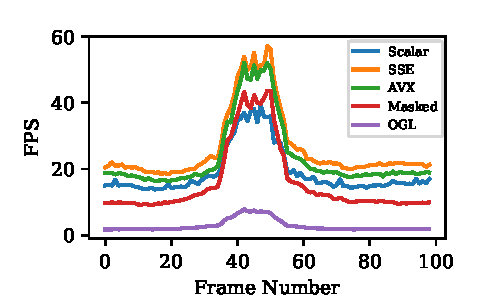
\includegraphics[width=\textwidth]{images/Evaluation_1_Results_FPS.pdf}
		\caption{Frame Number PDF}
	\end{minipage}
\end{figure}

\newpage
-
\section{Fazit}
Das ist ein Testsatz f"ur das Fazit.

\bibliographystyle{abbrv} 
%% use following if all content of bibtex file should be shown
% \nocite{*}
\bibliography{literatur}
\end{document}
